%%%%%%%%%%%%%%%%%%%%%%%%%%%%%%%%%%%%%%%%%
% University Assignment Title Page 
% LaTeX Template
% Version 1.0 (27/12/12)
%
% This template has been downloaded from:
% http://www.LaTeXTemplates.com
%
% Original author:
% WikiBooks (http://en.wikibooks.org/wiki/LaTeX/Title_Creation)
%
% License:
% CC BY-NC-SA 3.0 (http://creativecommons.org/licenses/by-nc-sa/3.0/)
% 
% Modified for COSC343 by:
% Lech Szymanski (5/5/2020)
%
% Adapted for AIML402 by:
% Lech Szymanski (18/7/2022)


\documentclass[12pt]{article}
\usepackage{cosc343style}


% Paper code -- change it to AIML402 if you're enrolled in AIML402
\papercode{COSC343}

% Your project title (change appropriately for the assignment)
\title{Assignment 1 report}

% Your name
\author{Luka \textsc{Didham}}
\studentid{7718477}


% Date, change the \today to a set date if you want to be precise
\reportdate{\today}

\begin{document}


\maketitle


\section{Introduction}

The purpose of this assignment is to create an an AI agent to play the game Wordle. Wordle is a word guessng game where the player must guess a five-letter word in six attempts.
Each time you guess, you're told whether the letters in your chosen word are in the target word, and whether they are in the right place. Traditionally the target word for the game is picked from a
dictionary of 2500 common English words. The assignment implementation differs by allowing game settings which allow multiple languages, varying word size, and includes much larger dictionaries.
Dictionaries in the implementation contain all words at a given word size for a given language resulting in very large dictionaries, with a English five-letter game having a dictionary of nearly 12,000 words.
The agent created is ranked by in how few moves it can correctly "guess" the target word, with a penalty that doubles the score if the agent does not guess the word within the variable maximum guess threshold.

\section{Implementation Overview}

My implementation supports all game settings and has varying performace between easy and hard mode discussed below. The agent has two main steps in which it repeats to find a target word.
\begin{itemize}
\item Filtering Remaining Dictionary: In this step we iterate through the entire remaining dictionary removing any words that can not be the target word. We decide if a word could be the possible target word based on the three factors of information detailed below. Each factor factor of information removes more words from our dictionary reducing our gussing averages. \begin{itemize}
            \item Letter state '1': These are letters found in the target word and in the correct position. This information is recorded in a Regex statement as a positive entry. The Regex is used to match remaining words in the dictionary. If any words do not match the Regex statment containing a letter state '1' in said postion the word will be deleted from the dictionary before the following guess.
      \end{itemize}
      \begin{itemize}
            \item Letter state '-1': These are letters found in the target word but in the incorrect position. This information is both recorded in a simple list "letters_included" and in the Regex statement as a negative not entry ([^XYZ]). The Regex is again used to match remaining words in the dictionary where if a word does contain the negative not letter in said postion it will be deleted. The list "letters_needed" is also iterated through for each word of the remaining dictionary. A word is removed if it does not contain all letters in the list "letters_needed"
      \end{itemize}
      \begin{itemize}
            \item Letter state '0': These are letters not found in the target word in any position. These letters are only added to the "letters_excluded" list. We then iterate through the remaining dictionary removing any words which contain any of these letters.
      \end{itemize}
\item Choosing From Remaining Dictionary
      \begin{itemize}
            \item Letter Frequency Ranking: After we have a filtered dictionary containing the least amount of words possible of being our target word we also rank them based on letter frequecny. Before every guess the agent will take the new dictionary and compiles a dictionary variable "dictionary_frequency" which contains a frequency for each letter. This process is done in the "LetterFrequencies" method where the method counts each time it sees a letter. As an example the contents "dictionary_frequency" may look like \{'A': 44355 ... 'Z': 18565\} where the letter "A" has been seen 44355 times and "Z" is seen 18565 times. These frequencies change as the dictionary is fitered so is updated each run. After we have letter frequencies we rank words in the remaing d
      \end{itemize}
\end{itemize}

You can use the \verb$\section{}$ and \verb$\subsection{}$ commands to organise your document - either break the main body into multiple sections, or have it as a one section with subsections.   \LaTeX{} handles all the formatting and numbering automatically. Use the \verb$\ref{}$ and \verb$\label{}$ commands for cross-references.  

\subsection{Citing}

You might want to cite some sources of your information.  For instance, a reference for \LaTeX{} can be found here \cite{latexcompanion}.

\subsection{How to compile \LaTeX{}}

\LaTeX{} documents are prepared using markup language and need to be compiled to produce pdfs.  

The easiest way is to use the \href{https://www.overleaf.com}{Overleaf service} - it's free for private projects.  Create an account and once you login you can create different projects (essentially different documents).  After clicking on ``New Project" select ``Upload project" and upload the \textit{cosc343report.zip} file where this file came from.  The template will open on the website and you'll be able to write your report through your browser, compile LaTeX online and have it saved on a remote server.  Later you just download the final pdf and submit as your report.    

Alternately, you can install LaTeX compiler on your machine and compile the .tex file yourself.  On macOS you need to download and install \href{http://www.tug.org/mactex/downloading.html}{MacTeX}.  Then, using a program like \href{http://pages.uoregon.edu/koch/texshop/}{TexShop} (free), or \href{https://www.texpad.com/}{Texpad} (awesome, but not free) you can edit and compile a .tex file into a .pdf.


\subsection{Tables and Figures}

Use the table and tabular commands for basic tables --- see Table~\ref{tab:widgets}, for example. You can include a figure (JPEG, PNG or PDF) with the \verb$\includegraphics$ command as in the code for Figure~\ref{fig:frog} below.

% Commands to include a figure:
\begin{figure}
\centering
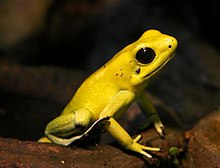
\includegraphics[width=0.4\textwidth]{figures/frog.jpg}
\caption{\label{fig:frog}This is a figure caption.}
\end{figure}

\begin{table}
\centering
\begin{tabular}{l|r}
Item & Quantity \\\hline
Widgets & 42 \\
Gadgets & 13
\end{tabular}
\caption{\label{tab:widgets}An example table.}
\end{table}

\subsection{Mathematics}

\LaTeX{} is great at typesetting mathematics. Let $X_1, X_2, \ldots, X_n$ be a sequence of independent and identically distributed random variables with $\text{E}[X_i] = \mu$ and $\text{Var}[X_i] = \sigma^2 < \infty$, and let
$$S_n = \frac{X_1 + X_2 + \cdots + X_n}{n}
      = \frac{1}{n}\sum_{i}^{n} X_i$$
denote their mean. Then as $n$ approaches infinity, the random variables $\sqrt{n}(S_n - \mu)$ converge in distribution to a normal $\mathcal{N}(0, \sigma^2)$.

\subsection{Lists}

You can make lists with automatic numbering \dots

\begin{enumerate}
\item Like this,
\item and this
\end{enumerate}
\dots or bullet points \dots
\begin{itemize}
\item Like this,
\item and this
\end{itemize}

\section{Conclusion}

Concluding remarks.  It could be a brief summary and/or comments on what you have learned/enjoyed/struggled with.      Depending on the space taken up by figures and formatting the report (excluding the Appendix) should be somewhere in the range of 3-5 pages.  Remember, it's not about creative space-wasting to hit the 4 pages, but about reporting on your work and results, so I can tell how much you have done and learned.  


%The environment \thebibliography produces a list of references; such list will be titled "References". A parameter inside braces, 3 in the example, indicates the number of entries to be added; this parameter can not be greater than 99.

%To create a bibliography entry the command \bibitem is used. A parameter inside braces is set to label this entry and can later be used as identifier for this reference. After the closing brace the text with the name of the author, the book title, publisher and so on is entered. 

%Any choice of citation style is acceptable as long as you are consistent.

\begin{thebibliography}{3}

\bibitem{latexcompanion} 
Michel Goossens, Frank Mittelbach, and Alexander Samarin. \textit{The \LaTeX\ Companion}. Addison-Wesley, Reading, Massachusetts, 1993.

\end{thebibliography}


% Activate the appendix
% from now on sections are numerated with capital letters
\appendix

\renewcommand{\thesection}{Appendix \Alph{section}}

\section{Some extra things}

If you have anything more to add you might want to add it to the appendix.  For instance, some details could detract from readability if placed in the main body of the report, but might still be needed in the appendix for completeness and/or reference.  You don't need to have an appendix if you don't think you need one.

\textbf{Do not stick code in the appendix} - any code should be submitted as a separate file (.py file for Python code).  


\end{document}